\documentclass[hyperref, a4paper]{article}

\usepackage{geometry}
\usepackage{titling}
\usepackage{titlesec}
% No longer needed, since we will use enumitem package
% \usepackage{paralist}
\usepackage{enumitem}
\usepackage{footnote}
% Conflicts with enumitem
%\usepackage{enumerate}
\usepackage{amsmath, amssymb, amsthm}
\usepackage{mathtools}
\usepackage{bbm}
\usepackage{cite}
\usepackage{graphicx}
\usepackage{subcaption}
\usepackage{physics}
\usepackage{tensor}
\usepackage{siunitx}
\usepackage[version=4]{mhchem}
\usepackage{tikz}
\usepackage{xcolor}
\usepackage{listings}
\usepackage{autobreak}
\usepackage[ruled, vlined, linesnumbered]{algorithm2e}
\usepackage{nameref,zref-xr}
\zxrsetup{toltxlabel}
%\zexternaldocument*[optics-]{../optics/optics}[optics.pdf]
%\zexternaldocument*[solid-]{../solid/solid}[solid.pdf]
\usepackage[colorlinks,unicode]{hyperref} % , linkcolor=black, anchorcolor=black, citecolor=black, urlcolor=black, filecolor=black
\usepackage[most]{tcolorbox}
\usepackage{prettyref}

% Page style
\geometry{left=3.18cm,right=3.18cm,top=2.54cm,bottom=2.54cm}
\titlespacing{\paragraph}{0pt}{1pt}{10pt}[20pt]
\setlength{\droptitle}{-5em}
\preauthor{\vspace{-10pt}\begin{center}}
\postauthor{\par\end{center}}

% More compact lists 
\setlist[itemize]{
    itemindent=17pt, 
    leftmargin=1pt,
    listparindent=\parindent,
    parsep=0pt,
}

% Math operators
\DeclareMathOperator{\timeorder}{\mathcal{T}}
\DeclareMathOperator{\diag}{diag}
\DeclareMathOperator{\legpoly}{P}
\DeclareMathOperator{\primevalue}{P}
\DeclareMathOperator{\sgn}{sgn}
\newcommand*{\ii}{\mathrm{i}}
\newcommand*{\ee}{\mathrm{e}}
\newcommand*{\const}{\mathrm{const}}
\newcommand*{\suchthat}{\quad \text{s.t.} \quad}
\newcommand*{\argmin}{\arg\min}
\newcommand*{\argmax}{\arg\max}
\newcommand*{\normalorder}[1]{: #1 :}
\newcommand*{\pair}[1]{\langle #1 \rangle}
\newcommand*{\fd}[1]{\mathcal{D} #1}
\DeclareMathOperator{\bigO}{\mathcal{O}}
\DeclareMathOperator{\li}{Li}

% TikZ setting
\usetikzlibrary{arrows,shapes,positioning}
\usetikzlibrary{calc}
\usetikzlibrary{arrows.meta}
\usetikzlibrary{decorations.markings}
\tikzstyle arrowstyle=[scale=1]
\tikzstyle directed=[postaction={decorate,decoration={markings,
    mark=at position .5 with {\arrow[arrowstyle]{stealth}}}}]
\tikzstyle ray=[directed, thick]
\tikzstyle dot=[anchor=base,fill,circle,inner sep=1pt]

% Algorithm setting
% Julia-style code
\SetKwIF{If}{ElseIf}{Else}{if}{}{elseif}{else}{end}
\SetKwFor{For}{for}{}{end}
\SetKwFor{While}{while}{}{end}
\SetKwProg{Function}{function}{}{end}
\SetArgSty{textnormal}

\newcommand*{\concept}[1]{{\textbf{#1}}}

% Embedded codes
\lstset{basicstyle=\ttfamily,
  showstringspaces=false,
  commentstyle=\color{gray},
  keywordstyle=\color{blue}
}

% Support for tensor double arrows.
\renewcommand{\tensor}[1]{ \stackrel{\leftrightarrow}{\vb*{#1}}}

% Reference formatting
\newrefformat{fig}{Figure~\ref{#1}}

% Color boxes
\tcbuselibrary{skins, breakable, theorems}
\newtcbtheorem[number within=section]{warning}{Warning}%
  {colback=orange!5,colframe=orange!65,fonttitle=\bfseries, breakable}{warn}
\newtcbtheorem[number within=section]{note}{Note}%
  {colback=green!5,colframe=green!65,fonttitle=\bfseries, breakable}{note}

\title{Mini Project Report}
\author{Jinyuan Wu}

\begin{document}

\maketitle

\begin{figure}
    \centering
    \begin{subfigure}{0.45\textwidth}
        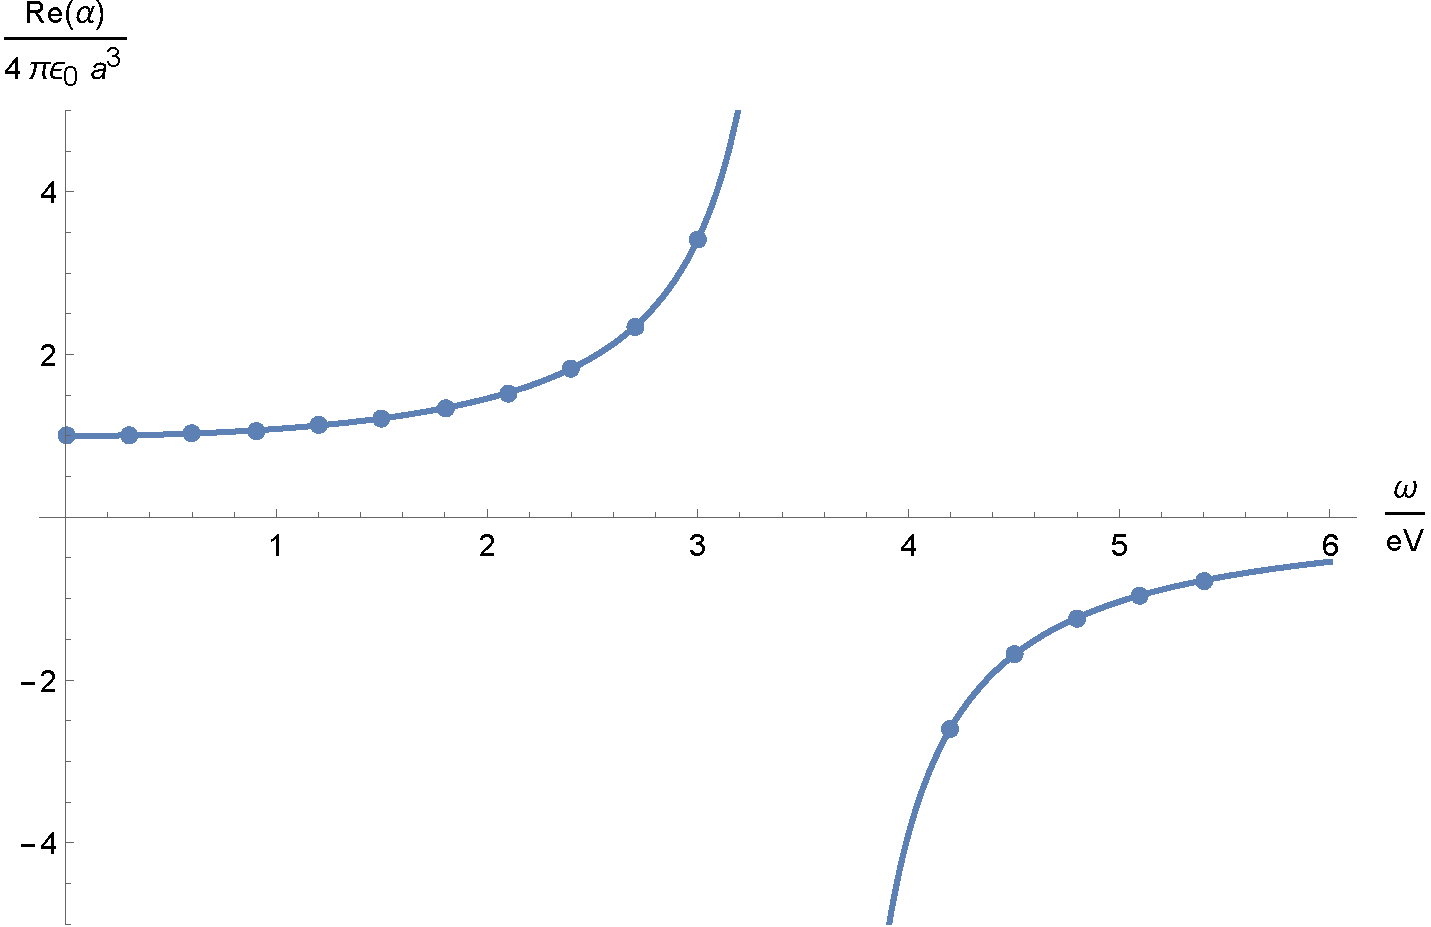
\includegraphics[width=\textwidth]{alpha-re.pdf}
        \subcaption{}
    \end{subfigure}
    \begin{subfigure}{0.45\textwidth}
        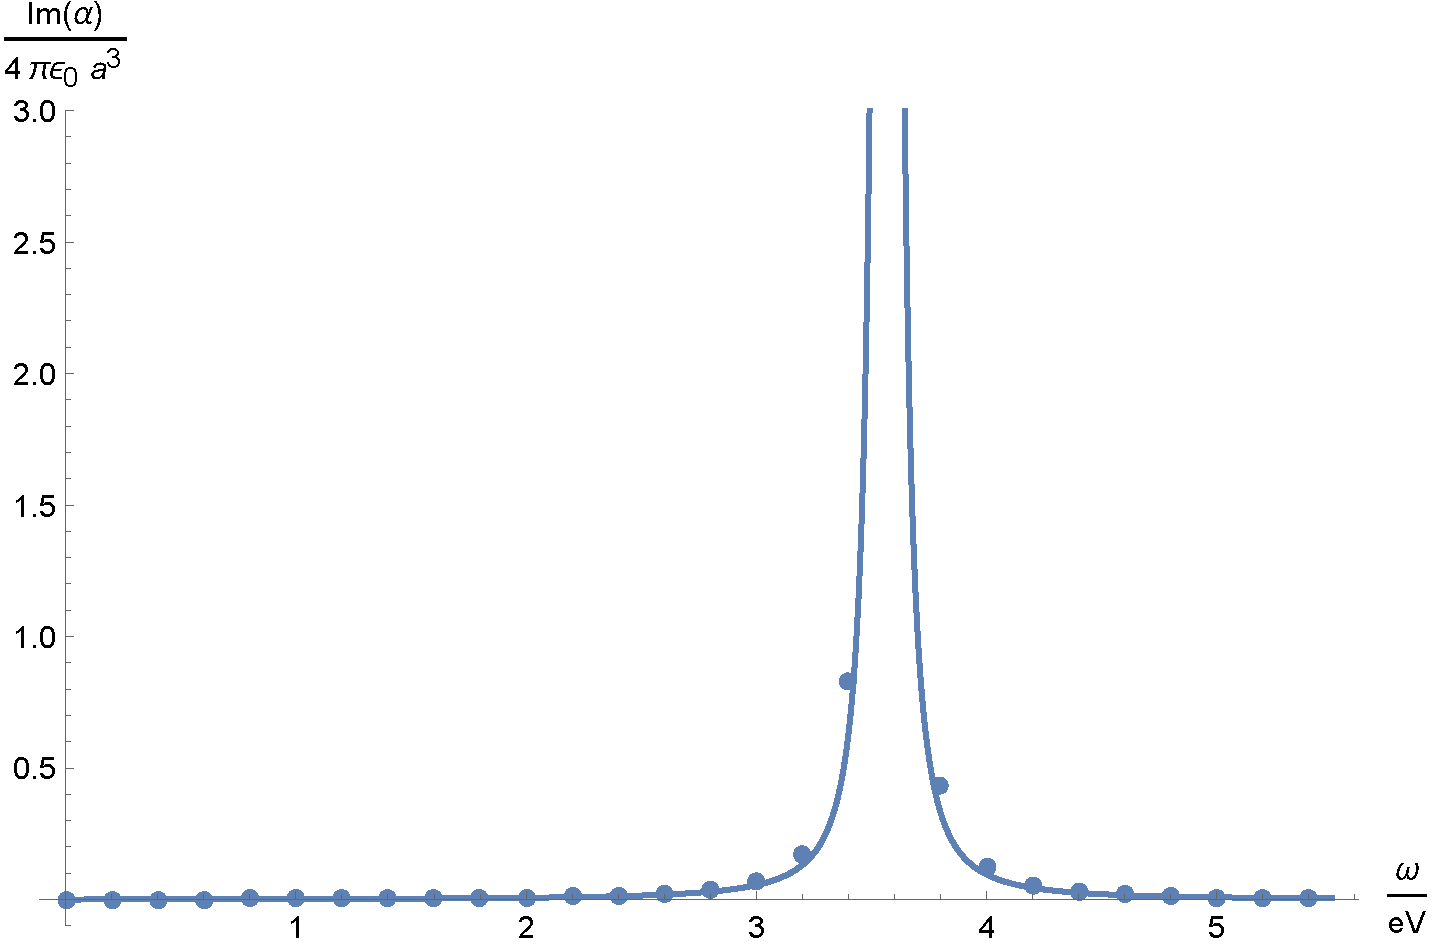
\includegraphics[width=\textwidth]{alpha-im.pdf}
        \subcaption{}
    \end{subfigure}
    \caption{The real and the imaginary part of $\alpha(\omega)$. The lines are plotted by definition, and the scattered points are obtained by K-K relations. (a) The real part. (b) The imaginary part.}
    \label{fig:plot}
\end{figure}

\paragraph{Problem 1} Consider a one dimensional infinite chain with the lattice constant $\Lambda$ on the $z$ direction consisting of metallic balls, 
each of which have radius $a$ and is made of a metal with permittivity
\begin{equation}
    \epsilon_\text{r} = 1 - \frac{\omega_\text{p}^2}{\omega (\omega + \ii \gamma)}.
\end{equation} 
When $a \to 0$, the polarizability of a single ball is 
\begin{equation}
    \alpha(\omega) = 4 \pi \epsilon_0 a^3 \frac{\epsilon_\text{r}(\omega) - 1}{\epsilon_\text{r}(\omega) + 2},
\end{equation}
We use Mathematica to plot the real and the imaginary part of $\alpha(\omega)$ and recalculate them with 
K-K relations 
\begin{equation}
    \Re \alpha(\omega) = - \frac{1}{\pi} \primevalue \int_{-\infty}^\infty \frac{\Im \alpha(\nu)}{\omega - \nu} \dd{\nu}, \quad \Im \alpha(\omega) = \frac{1}{\pi} \primevalue \int_{-\infty}^\infty \frac{\Re \alpha(\nu)}{\omega - \nu} \dd{\nu}
    \label{eq:kk-relation}
\end{equation}
in \prettyref{fig:plot}. It can be found that K-K relations do hold for $\alpha$. 

\begin{note*}{Numerical details of K-K relations}
    The prime value integral is implemented using the replacement 
    \[
        \primevalue \int_{-\infty}^\infty \longrightarrow \int_{-\infty}^{\omega - o} + \int_{\omega+o}^\infty,
    \]
    where $o \sim 0.01$ is a small number. If $o$ is too large, the peak of $\Im \alpha$ calculated by the 
    K-K relation will be broader than the exact value (see \prettyref{fig:plot}, where the scattered points 
    are slightly ``out'' of the exact peak). If $o$ is too small, there are severe convergence problems.
\end{note*}

Qualitatively, the behavior 
of $\alpha(\omega)$ is just like the behavior of the response of a driven damped oscillator, where the imaginary 
part diverges when $\epsilon_\text{r}(\omega) + 2 = 0$, or considering that $\gamma$ is small, when 
\begin{equation}
    \omega = \sqrt{\frac{1}{3}} \omega_\text{p} = \SI{3.56}{eV}.
\end{equation}
This frequency is the frequency of the local surface plasmon polariton of a single ball.
When the driving frequency is larger than $\omega_\text{p} / \sqrt{3}$, the real part of $\alpha$ is positive, 
which means the system is able to ``keep in track with'' the driving field. When $\omega > \omega_\text{p}$,
$\Re \alpha < 0$, which means that the system is too slow to response ``in time'' to the driving field and 
therefore has an opposite phase to the driving field.

\paragraph{}

\paragraph{Problem 2} We need to solve 
\begin{equation}
    \vb*{p}_m = \alpha (\vb*{E}_\text{ext}(\vb*{r}_m) + \omega^2 \mu_0 \sum_{n \neq m} \tensor{\vb*{G}}(\vb*{r}_m - \vb*{r}_n) \cdot \vb*{p}_n),
    \label{eq:p-ext}
\end{equation}
and when there is no external field, by the Bloch condition 
\begin{equation}
    \vb*{p}_m = \vb*{u} \ee^{\ii k z_m},
\end{equation}
we have 
\[
    \vb*{u} \ee^{\ii k z_m} = \alpha \omega^2 \mu_0 \sum_{n \neq m} \tensor{\vb*{G}}(\vb*{r}_m - \vb*{r}_n) \cdot \vb*{u} \ee^{\ii k z_n},
\]
\[
    \left( \tensor{\vb*{I}} - \alpha \omega^2 \mu_0 \sum_{n \neq m} \tensor{\vb*{G}}(\vb*{r}_m - \vb*{r}_n) \ee^{\ii k z_n} \ee^{- \ii k z_m}  \right) \vb*{u}  = 0,
\]
and we have 
\begin{equation}
    \tensor{\vb*{M}} = \alpha^{-1} \tensor{ \vb*{I}} - \omega^2 \mu_0 \sum_{n \neq m} \tensor{\vb*{G}}(\vb*{r}_m - \vb*{r}_n) \ee^{\ii k (z_n - z_m)}, \quad \tensor{\vb*{M}} \vb*{u} = 0,
    \label{eq:eigen-problem}
\end{equation}
and we need to evaluate 
\begin{equation}
    \tensor{\vb*{W}} = \omega^2 \mu_0 \sum_{n \neq m} \tensor{\vb*{G}}(\vb*{r}_m - \vb*{r}_n) \ee^{\ii k (z_n - z_m)}.
    \label{eq:def-w}
\end{equation}

The dyadic Green function is 
\begin{equation}
    \tensor{G}(\vb*{R}) = \frac{k_0}{4\pi} \frac{\ee^{\ii k_0 R}}{k_0 R} \Biggl( \tensor{I} \left( 1 - \frac{4\pi R}{3k_0^2} \delta(\vb*{R}) - \frac{1}{k_0^2 R^2} + \frac{\ii}{k_0 R} \right) 
        + \frac{\vb*{R} \vb*{R}}{R^2} \left( \frac{3}{k_0^2 R^2} - 1 - \frac{3\ii}{k_0 R} \right) \Biggr).
\end{equation}
Since $\vb*{R} = \vb*{r}_m - \vb*{r}_n \neq 0$, the $\delta$-function term vanishes. Since $\vb*{r}_m - \vb*{r}_n$
is along the $z$ axis, We have 
\[
    \frac{\vb*{R} \vb*{R}}{R^2} = \vb*{e}_z \vb*{e}_z, \quad R = \abs*{z_m - z_n}.
\]
Therefore, by the definition \eqref{eq:def-w}, we have 
\[
    \begin{aligned}
        \tensor{\vb*{W}} &= \omega^2 \mu_0 \sum_{m \neq n} \ee^{\ii k(z_n - z_m)} \frac{k_0}{4\pi} \ee^{\ii k_0 R}
        \Biggl( \tensor{\vb*{I}} \left( \frac{1}{k_0 R} + \frac{\ii}{k_0^2 R^2} - \frac{1}{k_0^3 R^3} \right) \\
        &\quad \quad + \vb*{e}_z \vb*{e}_z \left( - \frac{1}{k_0 R} - \frac{3 \ii}{k_0^2 R^2} + \frac{3}{k_0^3 R^3} \right) \Biggr) \\
        &= \omega^2 \mu_0 \frac{k_0}{4\pi} \left( \sum_{z_m < z_n} + \sum_{z_m > z_n} \right) \ee^{\ii k_0 R - \ii k (z_m - z_n)} \Biggl( \tensor{\vb*{I}} \left( \frac{1}{k_0 R} + \frac{\ii}{k_0^2 R^2} - \frac{1}{k_0^3 R^3} \right) \\
        &\quad \quad + \vb*{e}_z \vb*{e}_z \left( - \frac{1}{k_0 R} - \frac{3 \ii}{k_0^2 R^2} + \frac{3}{k_0^3 R^3} \right) \Biggr) \\ 
        &= \omega^2 \mu_0 \frac{k_0}{4\pi} \left( \sum_{l=1}^\infty \ee^{\ii (k_0 - k) \Lambda l} + \sum_{l=1}^\infty \ee^{\ii (k_0 + k) \Lambda l} \right) \Biggl( \tensor{\vb*{I}} \left( \frac{1}{k_0 \Lambda l} + \frac{\ii}{k_0^2 \Lambda^2 l^2} - \frac{1}{k_0^3 \Lambda^3 l^3} \right) \\
        &\quad \quad + \vb*{e}_z \vb*{e}_z \left( - \frac{1}{k_0 \Lambda l} - \frac{3 \ii}{k_0^2 \Lambda^2 l^2} + \frac{3}{k_0^3 \Lambda^3 l^3} \right) \Biggr) .
    \end{aligned}
\] 
Using formulae from \href{https://en.wikipedia.org/wiki/Polylogarithm}{Wikipedia}, we have 
\[
    \left( \sum_{l=1}^\infty \ee^{\ii (k_0 - k) \Lambda l} + \sum_{l=1}^\infty \ee^{\ii (k_0 + k) \Lambda l} \right) \frac{1}{l^s} = \li_s(\ee^{\ii (k_0 - k) \Lambda}) + \li_s(\ee^{\ii (k_0 + k) \Lambda}),
\]
So finally we have 
\begin{equation}
    \begin{aligned}
        \tensor{\vb*{W}} &= \frac{\omega^2 \mu_0 k_0}{4 \pi} \biggl(
        \frac{1}{k_0 \Lambda} (\tensor{\vb*{I}} - \vb*{e}_e \vb*{e}_z) (\li_1(\ee^{\ii (k_0 - k) \Lambda}) + \li_1(\ee^{\ii (k_0 + k) \Lambda})) \\
        &\quad \quad + \frac{\ii}{k_0^2 \Lambda^2} (\tensor{\vb*{I}} - 3 \vb*{e}_z \vb*{e}_z) (\li_2(\ee^{\ii (k_0 - k) \Lambda}) + \li_2(\ee^{\ii (k_0 + k) \Lambda})) \\
        &\quad \quad - \frac{1}{k_0^3 \Lambda^3} (\tensor{\vb*{I}} - 3 \vb*{e}_z \vb*{e}_z) (\li_3(\ee^{\ii (k_0 - k) \Lambda}) + \li_3(\ee^{\ii (k_0 + k) \Lambda})).
        \biggr)
    \end{aligned}
    \label{eq:w-explicit}
\end{equation}

\paragraph{}

\paragraph{Problem 3} When the system is in a single mode, we have $\vb*{p}_m = \alpha_\text{eff} 
\vb*{E}_\text{eig}$, and from \eqref{eq:p-ext} we have 
\[
    \alpha^{-1} \vb*{p}_m = \alpha_\text{eig}^{-1} \vb*{p}_m + \omega^2 \mu_0 \sum_{n \neq m} \tensor{\vb*{G}}(\vb*{r}_m - \vb*{r}_n) \cdot \vb*{p}_n,
\]
and we find it is equivalent to 
\begin{equation}
    \tensor{\vb*{M}} \cdot \ \vb*{u} = \frac{1}{\alpha_\text{eff}} \vb*{u} = \lambda \vb*{u}.
    \label{eq:external-eigen}
\end{equation}
The eigenvalues are inverse effective polarizabilities. \eqref{eq:external-eigen} is equivalent to 
\[
    \alpha^{-1} \vb*{u} \ - \tensor{\vb*{W}} \cdot \ \vb*{u} = \alpha_\text{eig}^{-1} \vb*{u},
\]
and we known that $\tensor{\vb*{W}}$ is diagonal in the $\vb*{e}_x, \vb*{e}_y, \vb*{e}_z$ basis, so the
eigenvectors - which are polarization directions - are just $\vb*{e}_x, \vb*{e}_y, \vb*{e}_z$, and it is straightforward to find that the 
polarizabilities on the $x$ and $y$ directions are the same: 
\begin{equation}
    \begin{aligned}
        \alpha_\text{eig,$xy$}^{-1} &= \alpha^{-1} - \frac{\omega^2 \mu_0 k_0}{4 \pi} \biggl( \frac{1}{k_0 \Lambda} (\li_1(\ee^{\ii (k_0 - k) \Lambda}) + \li_1(\ee^{\ii (k_0 + k) \Lambda})) \\
        &\quad \quad + \frac{\ii}{k_0^2 \Lambda^2} (\li_2(\ee^{\ii (k_0 - k) \Lambda}) + \li_2(\ee^{\ii (k_0 + k) \Lambda})) - \frac{1}{k_0^3 \Lambda^3} (\li_3(\ee^{\ii (k_0 - k) \Lambda}) + \li_3(\ee^{\ii (k_0 + k) \Lambda})) \biggr),
    \end{aligned}
    \label{eq:alpha-xy}
\end{equation}
and the polarizability on the $z$ direction is 
\begin{equation}
    \begin{aligned}
        \alpha_\text{eig,$z$}^{-1} &= \alpha^{-1} - \frac{\omega^2 \mu_0 k_0}{4 \pi} \biggl( - \frac{2\ii}{k_0^2 \Lambda^2} (\li_2(\ee^{\ii (k_0 - k) \Lambda}) + \li_2(\ee^{\ii (k_0 + k) \Lambda})) \\
        &\quad \quad  + \frac{2}{k_0^3 \Lambda^3} (\li_3(\ee^{\ii (k_0 - k) \Lambda}) + \li_3(\ee^{\ii (k_0 + k) \Lambda})) \biggr).
    \end{aligned}
    \label{eq:alpha-z}
\end{equation}

Plotting \eqref{eq:alpha-xy} and \eqref{eq:alpha-z} on the complex plane, we get \prettyref{fig:complex-plane}.
It can be found that between \SI{3}{eV} and \SI{4}{eV}, $\Im \alpha$ is considerably large, indicating that 
there are bands of eigenmodes in this frequency range. This frequency range is close to $\omega_\text{p} / 
\sqrt{3}$, which means these eigenmodes are modified (since there is a periodic lattice, and dipoles interact
with each other) local surface plasmon polariton modes. The behaviors of the $x$- and $y$-polarized modes are 
the same, which is expected because of the rotational symmetry around the $z$ axis.

We also see two V-shaped blank regions in the plots,
which means there are singularities along two $\omega=ak$ lines. These singularity lines come from the fact 
that $\li_s z$ is actually a multi-valued function, and its principal branch has a branch cut $1 < z < \infty$.
When $k_0$ is close to $k$, $\ee^{\ii (k_0 - k) \Lambda}$ is close to $1$. 
In \prettyref{fig:all} we plot the points where $k_0 = k$ onto \prettyref{fig:complex-plane}, and it can be 
seen that these points determine the position of the V-shaped blank regions.

We find that there is no $1 / k_0 \Lambda$ term in \eqref{eq:alpha-z}, because it is a longitude mode
(the polarization direction is the same as the direction of the wave vector), while 
the $\sim 1/r$ term in the electric field generated by an oscillating dipole corresponds to the far-field 
electromagnetic wave behavior, which is definitely not a longitude mode. 

\begin{figure}
    \centering
    \begin{subfigure}{0.45\textwidth}
        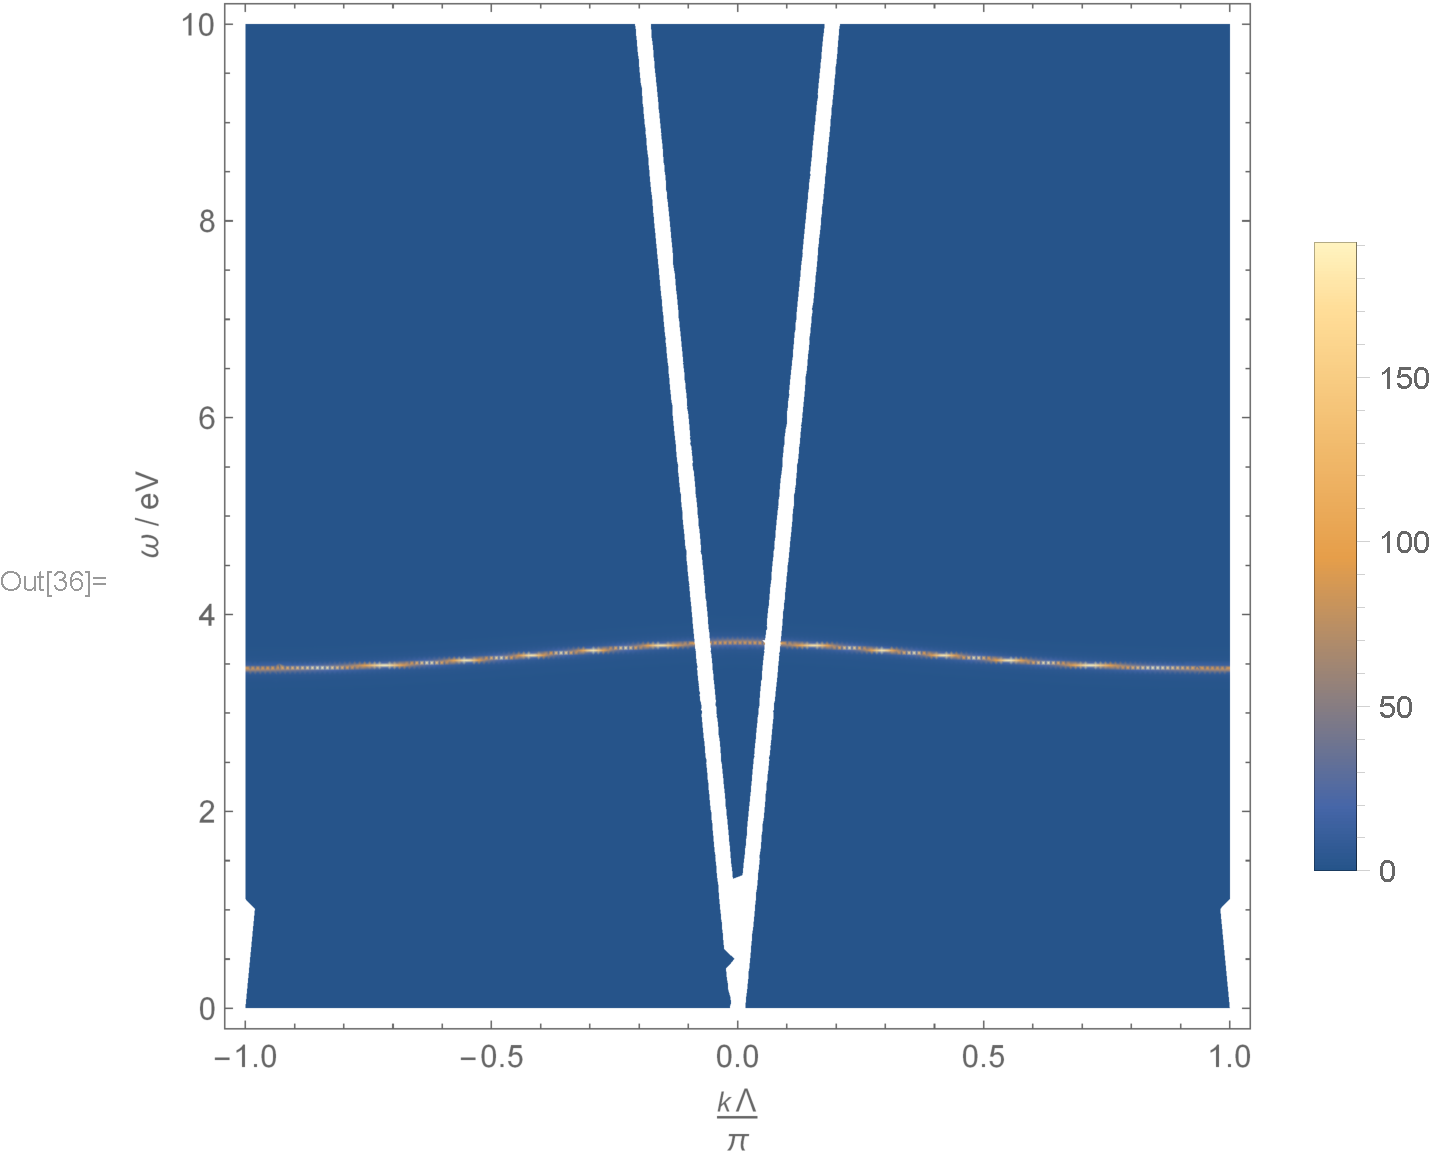
\includegraphics[width=\textwidth]{alphaxy-complex-plane.pdf}
        \subcaption{$\alpha_{xy}$}
    \end{subfigure}
    \begin{subfigure}{0.45\textwidth}
        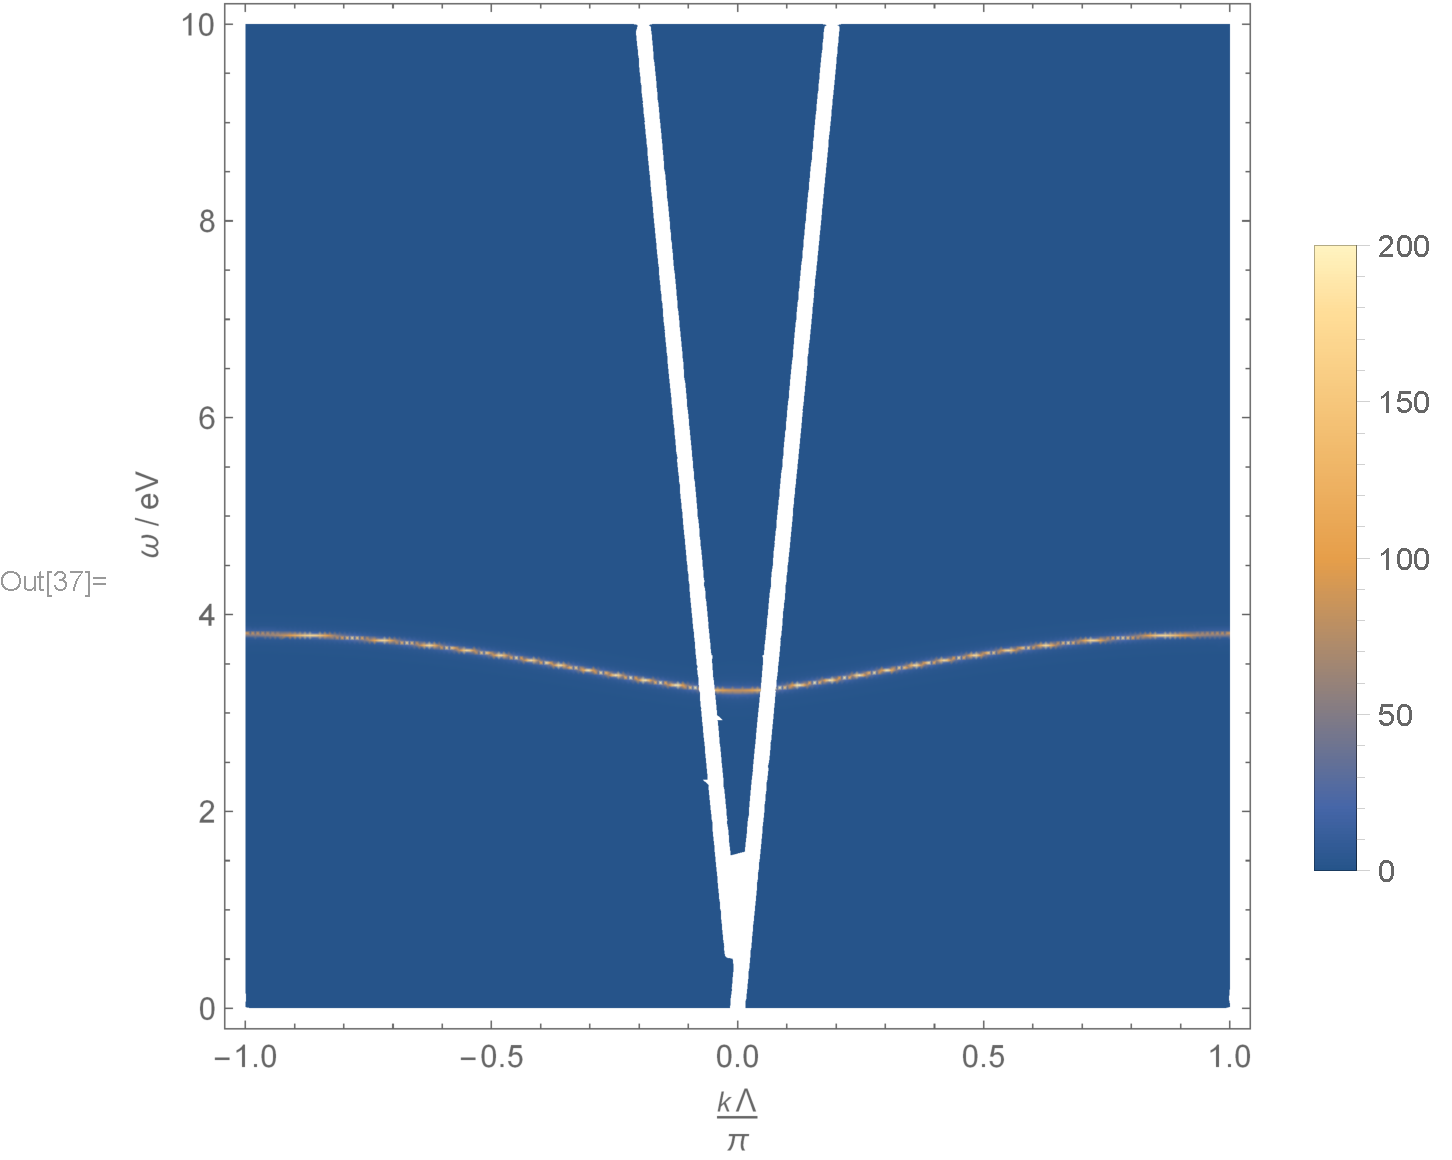
\includegraphics[width=\textwidth]{alphaz-complex-plane.pdf}
        \subcaption{$\alpha_{z}$}
    \end{subfigure}
    \caption{$\alpha_{xy}(\omega)$ and $\alpha_z(\omega)$ on the complex plane. }
    \label{fig:complex-plane}
\end{figure} 

\paragraph{}

\paragraph{Problem 4} In the $c \to \infty$ limit, $k_0 \to 0$, so all $1 / (k_0 \Lambda)^s$ terms in \eqref{eq:w-explicit} diverges,
and only the most divergent terms where $s=3$ are important, i.e. we only keep the near field terms 
in $\tensor{\vb*{G}}$, and we have 
\[
    \tensor{\vb*{W}} = \omega^2 \frac{\mu_0 k_0}{4 \pi} \left( \frac{3 \vb*{e}_z \vb*{e}_z - \tensor{\vb*{I}}}{k_0^3 \Lambda^3} \right) (\li_3(\ee^{\ii k \Lambda}) + \li_3 (\ee^{- \ii k \Lambda})).
\] 
In the $\gamma \to 0$ limit, we have 
\[
    \frac{1}{\alpha} = \frac{1}{4 \pi \epsilon_0 a^3} \frac{\epsilon_\text{r} + 2}{\epsilon_\text{r} - 1}
    = \frac{1}{4 \pi \epsilon_0 a^3} \frac{\omega_\text{p}^2 - 3 \omega^2}{\omega_\text{p}^2}. 
\]
So $\tensor{\vb*{W}} \cdot \ \vb*{u} = \vb*{u} / \alpha$ can be written as
\[
    \frac{1}{\alpha} = \frac{1}{4 \pi \epsilon_0 a^3} \frac{\omega_\text{p}^2 - 3 \omega^2}{\omega_\text{p}^2} \vb*{u} = \underbrace{\omega^2 \frac{\mu_0 }{4 \pi} \frac{1}{k_0^2}}_{= \frac{\mu_0 c^2}{4\pi} = \frac{1}{4 \pi \epsilon_0}} \left( \frac{3 \vb*{e}_z \vb*{e}_z - \tensor{\vb*{I}}}{ \Lambda^3} \right) (\li_3(\ee^{\ii k \Lambda}) + \li_3 (\ee^{- \ii k \Lambda})) \vb*{u},
\]
and finally  
\begin{equation}
    \tensor{\vb*{H}} \cdot \ \vb*{u} = \frac{\omega^2}{\omega_\text{p}^2} \vb*{u},
\end{equation}
where 
\begin{equation}
    \tensor{\vb*{H}} = \frac{1}{3} \left(1 - \frac{a^3}{\Lambda^3} (3 \vb*{e}_z \vb*{e}_z - \tensor{\vb*{I}}) (\li_3(\ee^{\ii k \Lambda}) + \li_3 (\ee^{- \ii k \Lambda})) \right) .
    \label{eq:eff-ham}
\end{equation}
By definition we know that $(\li_3(\ee^{\ii k \Lambda}) + \li_3 (\ee^{- \ii k \Lambda}))$ is a real number, so 
\eqref{eq:eff-ham} is a Hermitian matrix, and therefore qualifies as a Hamiltonian. Again, we find that 
$\tensor{\vb*{H}}$'s eigenvectors are $\vb*{e}_x$, $\vb*{e}_y$ and $\vb*{e}_z$ (the same as Problem 3), and the eigenvalues are 
\begin{equation}
    \frac{\omega_{xy}^2}{\omega_\text{p}^2} = \frac{1}{3} \left( 1 + \frac{a^3}{\Lambda^3} (\li_3(\ee^{\ii k \Lambda}) + \li_3 (\ee^{- \ii k \Lambda})) \right) ,
    \label{eq:omega-xy}
\end{equation}
and 
\begin{equation}
    \frac{\omega_{z}^2}{\omega_\text{p}^2} = \frac{1}{3} \left( 1 - \frac{2a^3}{\Lambda^3} (\li_3(\ee^{\ii k \Lambda}) + \li_3 (\ee^{- \ii k \Lambda})) \right) .
    \label{eq:omega-z}
\end{equation}
These dispersion relations are plotted as \prettyref{fig:omega}. 

\begin{figure}
    \centering
    \begin{subfigure}{0.45\textwidth}
        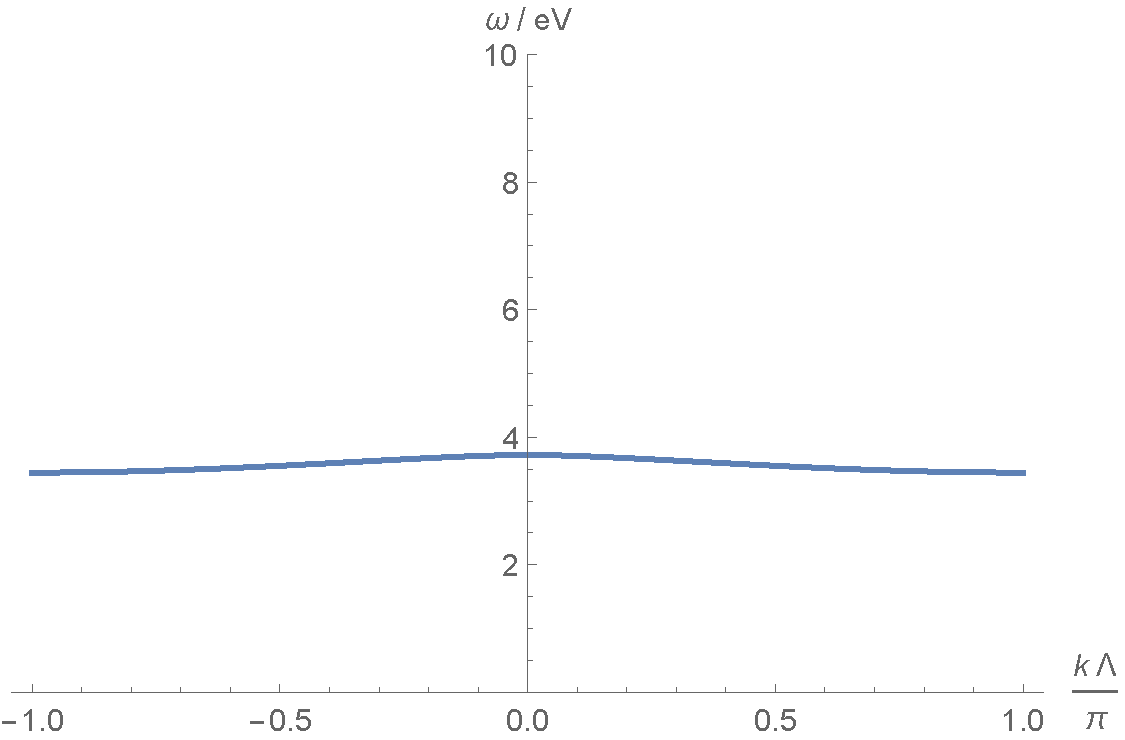
\includegraphics[width=\textwidth]{omegaxy.pdf}
        \subcaption{$\omega_{xy}$}
    \end{subfigure}
    \begin{subfigure}{0.45\textwidth}
        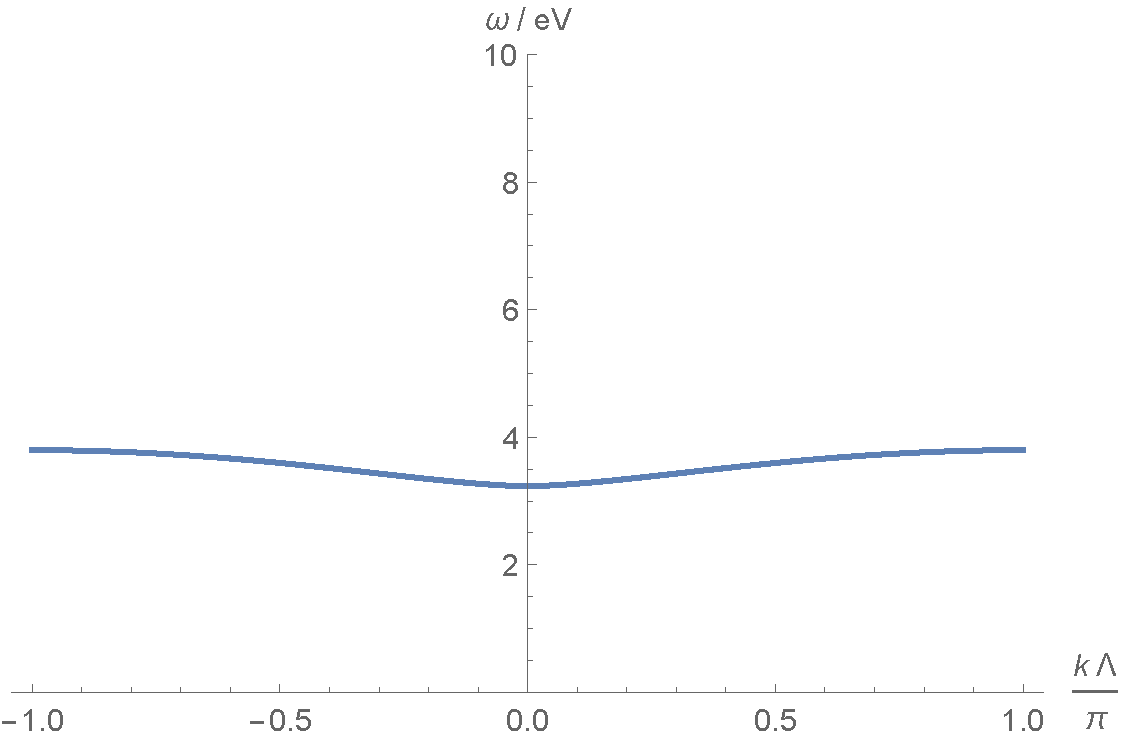
\includegraphics[width=\textwidth]{omegaz.pdf}
        \subcaption{$\omega_z$}
    \end{subfigure}
    \caption{Dispersion relations \eqref{eq:omega-xy} and \eqref{eq:omega-z}.}
    \label{fig:omega}
\end{figure}

Plotting the dispersion relations and the singularity points into \prettyref{fig:complex-plane}, we get 
\prettyref{fig:all}. It can be seen that $\alpha$ is significantly large at the dispersion relation curves,
as is expected. The features of the dispersion relations have been discussed in Problem 3. The reason why 
the quasi-stationary approximation works well here is because for the quasi-stationary approximation to work we need 
\[
    \hbar \omega \ll \frac{2 \pi c \hbar}{\Lambda} = \SI{16.5}{eV},
\]
and for $\omega$ around $\omega_\text{p} / \sqrt{3}$ this is not a bad approximation. 

\begin{figure}
    \centering
    \begin{subfigure}{0.45\textwidth}
        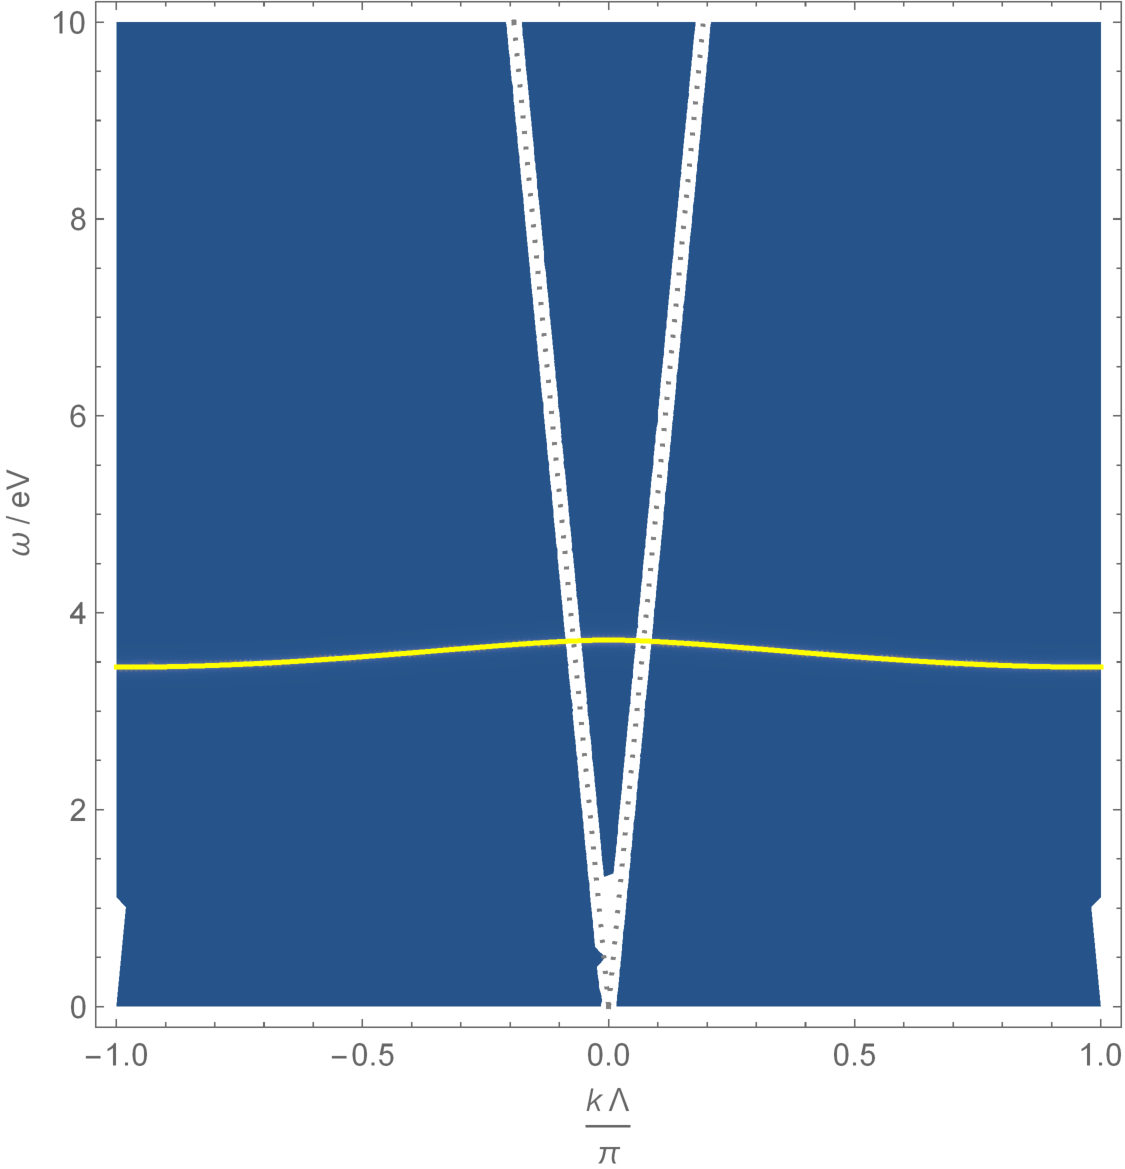
\includegraphics[width=\textwidth]{alphaxy-annotated.pdf}
        \subcaption{$\alpha_{xy}$}
    \end{subfigure}
    \begin{subfigure}{0.45\textwidth}
        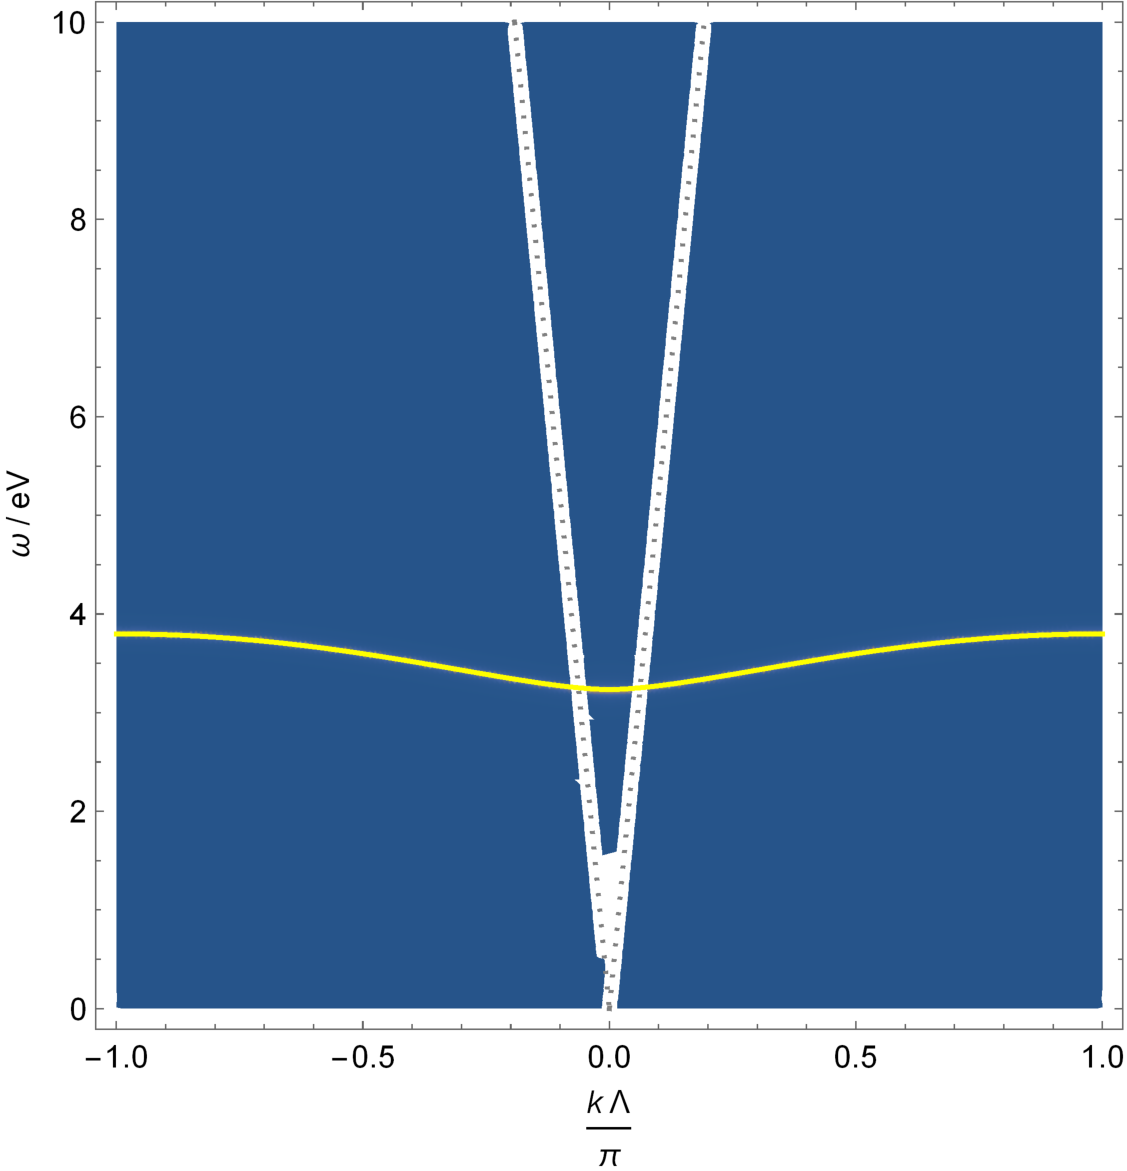
\includegraphics[width=\textwidth]{alphaz-annotated.pdf}
        \subcaption{$\alpha_z$}
    \end{subfigure}
    \caption{$\Im \alpha$ on the complex plane, with the dispersion relations (the yellow line) obtained from the 
    quasi-stationary approximation and the singularity points (the gray dotted lines) annotated.}
    \label{fig:all}
\end{figure}

The fact that all collective modes can be obtained using the quasi-stationary approximation also explains the 
shape of the dispersion relations. We can just regard the electric field generated by a single dipole as the 
electric field of a (quasi)-static dipole. For the $x$- or $y$-polarized mode, a dipole induces another dipole 
in the balls nearby that has the opposite direction with itself (see \prettyref{fig:dipole-field}(a)), while 
for a $z$-polarized mode, a dipole induces another dipole in the balls nearby that has the same direction with
itself (see \prettyref{fig:dipole-field}(b)). In other words, in $x$- and $y$-polarized modes, a dipole 
\emph{suppresses} dipoles nearby, while in the $z$-polarized modes, a dipole \emph{enhances} dipoles nearby.
For a 1D oscillator chain 
\[
    \ddot{x}_n = - \omega_0^2 + K(x_{n+1} + x_{n-1} - 2 x_n),
\]
where $K > 0$ means an oscillator lifts the neighbors, while $K < 0$ means an oscillator suppresses the neighbors,
the periodic solution is 
\begin{equation}
    x_n = A \ee^{\ii k \Lambda n - \ii \omega t}, \quad \omega^2 = \omega_0^2 + 2K (1 - \cos (k \Lambda)),
\end{equation}
so if $K > 0$, $\omega$ increases when $k$ increases, and when $K<0$ it is exactly the opposite.
This explains why for $x$- and $y$-polarized modes, as $k$ goes up, $\omega$ decreases, while for $z$-polarized 
modes, as $k$ goes up, $\omega$ increases.

\begin{figure}
    \centering
    

\tikzset{every picture/.style={line width=0.75pt}} %set default line width to 0.75pt        

\begin{tikzpicture}[x=0.75pt,y=0.75pt,yscale=-0.7,xscale=0.7]
%uncomment if require: \path (0,355); %set diagram left start at 0, and has height of 355

%Image [id:dp962691846432673] 
\draw (515.5,222.5) node  {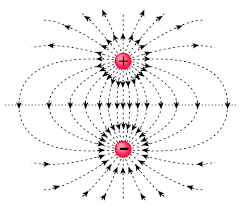
\includegraphics[width=99.75pt,height=99.75pt]{dipole-field.png}};
%Straight Lines [id:da6792737911619806] 
\draw    (517,277) -- (517,29.4) ;
\draw [shift={(517,27.4)}, rotate = 90] [fill={rgb, 255:red, 0; green, 0; blue, 0 }  ][line width=0.08]  [draw opacity=0] (12,-3) -- (0,0) -- (12,3) -- cycle    ;
%Straight Lines [id:da4136268135430723] 
\draw [color={rgb, 255:red, 74; green, 144; blue, 226 }  ,draw opacity=1 ][line width=1.5]    (517,251) -- (517,198.4) ;
\draw [shift={(517,194.4)}, rotate = 90] [fill={rgb, 255:red, 74; green, 144; blue, 226 }  ,fill opacity=1 ][line width=0.08]  [draw opacity=0] (15.6,-3.9) -- (0,0) -- (15.6,3.9) -- cycle    ;
%Straight Lines [id:da5882193234619546] 
\draw [color={rgb, 255:red, 74; green, 144; blue, 226 }  ,draw opacity=1 ][line width=1.5]    (517,127.4) -- (517,74.79) ;
\draw [shift={(517,70.79)}, rotate = 90] [fill={rgb, 255:red, 74; green, 144; blue, 226 }  ,fill opacity=1 ][line width=0.08]  [draw opacity=0] (15.6,-3.9) -- (0,0) -- (15.6,3.9) -- cycle    ;
%Straight Lines [id:da21684822857397124] 
\draw [color={rgb, 255:red, 80; green, 227; blue, 194 }  ,draw opacity=1 ][line width=1.5]    (504,122) -- (504,84.4) ;
\draw [shift={(504,80.4)}, rotate = 90] [fill={rgb, 255:red, 80; green, 227; blue, 194 }  ,fill opacity=1 ][line width=0.08]  [draw opacity=0] (15.6,-3.9) -- (0,0) -- (15.6,3.9) -- cycle    ;

%Image [id:dp5512957233213471] 
\draw (183.5,143.5) node  {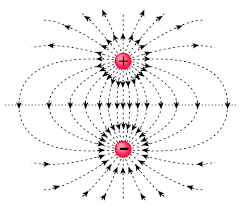
\includegraphics[width=99.75pt,height=99.75pt]{dipole-field.png}};
%Straight Lines [id:da5660597373419685] 
\draw    (67,144) -- (332,144) ;
\draw [shift={(334,144)}, rotate = 180] [fill={rgb, 255:red, 0; green, 0; blue, 0 }  ][line width=0.08]  [draw opacity=0] (12,-3) -- (0,0) -- (12,3) -- cycle    ;
%Straight Lines [id:da2620319569768228] 
\draw [color={rgb, 255:red, 74; green, 144; blue, 226 }  ,draw opacity=1 ][line width=1.5]    (185,172) -- (185,119.4) ;
\draw [shift={(185,115.4)}, rotate = 90] [fill={rgb, 255:red, 74; green, 144; blue, 226 }  ,fill opacity=1 ][line width=0.08]  [draw opacity=0] (15.6,-3.9) -- (0,0) -- (15.6,3.9) -- cycle    ;
%Straight Lines [id:da16953873290054022] 
\draw [color={rgb, 255:red, 80; green, 227; blue, 194 }  ,draw opacity=1 ][line width=1.5]    (272,160) -- (272,122.4) ;
\draw [shift={(272,164)}, rotate = 270] [fill={rgb, 255:red, 80; green, 227; blue, 194 }  ,fill opacity=1 ][line width=0.08]  [draw opacity=0] (15.6,-3.9) -- (0,0) -- (15.6,3.9) -- cycle    ;
%Straight Lines [id:da8731747530295029] 
\draw [color={rgb, 255:red, 74; green, 144; blue, 226 }  ,draw opacity=1 ][line width=1.5]    (280,172) -- (280,119.4) ;
\draw [shift={(280,115.4)}, rotate = 90] [fill={rgb, 255:red, 74; green, 144; blue, 226 }  ,fill opacity=1 ][line width=0.08]  [draw opacity=0] (15.6,-3.9) -- (0,0) -- (15.6,3.9) -- cycle    ;

% Text Node
\draw (529,20.4) node [anchor=north west][inner sep=0.75pt]    {$z\ \text{mode}$};
% Text Node
\draw (207,320) node [anchor=north west][inner sep=0.75pt]   [align=left] {(a)};
% Text Node
\draw (509,320) node [anchor=north west][inner sep=0.75pt]   [align=left] {(b)};
% Text Node
\draw (336,144) node [anchor=west] [inner sep=0.75pt]    {$x,y\ \text{modes}$};


\end{tikzpicture}

    \caption{The interaction between dipoles: a dipole (blue arrow) induces another dipole (green arrow) in balls nearby. (a) The case of $x$- or $y$-polarized mode. (b) The case of $z$-polarized mode. }
    \label{fig:dipole-field}
\end{figure}

\end{document}